\section*{Hardware structure}
\section*{Ion propulsion system}
\hspace{\parindent}Three primary parts make up an ion propulsion system: an air gap, an emitter wire (corona), and a downstream-positioned collector wire or strip. For maximum thrust and the achievement of a saturated corona current condition, the emitter and collector should be positioned as close to each other as feasible to create a narrow air gap but ensure there will be
no arcing\cite{cichocki2017electric}. The ionocraft structure and a high-voltage power supply are the two main parts of an ionocraft. The particular implementation phases depend on whether the ionocraft structure is exposed-coupled (corona) or exposed-decoupled (DBD).
\subsection*{High voltage power supply}
\hspace{\parindent}The electrical energy required to produce ionized air and drive the ionocraft is supplied by the high-voltage power source. Although alternating current (AC) and direct current (DC) power sources can be utilized, DC power supplies are typically chosen because of their efficiency and simplicity.
\subsubsection*{DC power source:}
\begin{wrapfigure}{r}{0.5\textwidth} %this figure will be at the right
    \centering
    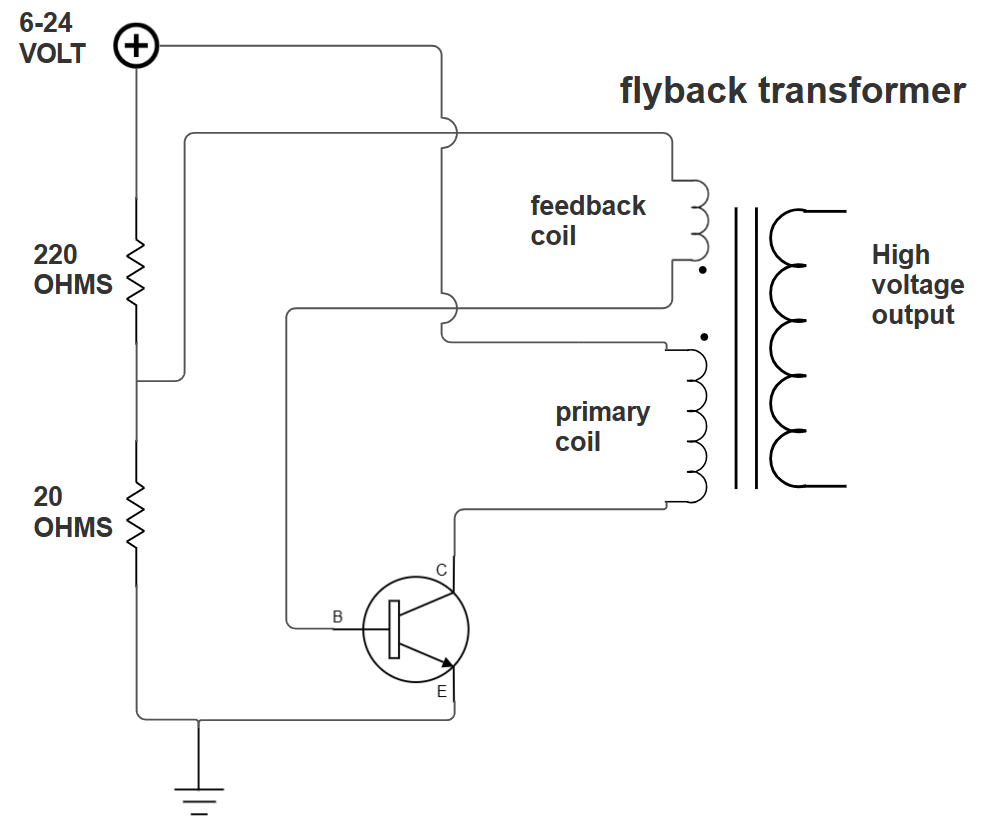
\includegraphics[width=0.5\textwidth]{images/circuit.PNG}
    \caption{Implementation circuit of high voltage generator}
\end{wrapfigure}
\hspace{\parindent}Typical components of a DC high-voltage power supply include the following:\\
• Low voltage power supply: Offers 6 to 24 volts as an input voltage.\\
• Transistor: Controls the flow of current.\\
• Voltage divider: Splits the voltage to get the appropriate amount.\\
• Flyback Transformer: Increases input voltage to the necessary high voltage level step by step.Older cathode-ray tube (CRT) televisions frequently include flyback transformers.\\\\
\subsection*{Structure of ionocraft}
\hspace{\parindent}The actual configuration of the electrodes that produce ionized air is referred to as the ionocraft structure. The "lifter" which usually comprises a triangular or circular frame with a suspended corona wire (thin wire electrode) above it, is the most basic sort of ionocraft structure. The collector electrode is the frame.
\subsubsection*{Coupled vs Decoupled}
\hspace{\parindent}There are two types of simple lifters: coupled and decoupled. The collector electrode and corona wire of a coupled ionocraft are connected directly to the high-voltage power supply. Although it is simpler to use, this kind of ionocraft might be less effective and more prone to instability\cite{drew2018toward}. A decoupled ionocraft, on the other hand, controls the voltage provided to the corona wire using a different control circuit. Although they are more difficult to operate, decoupled ionocrafts can provide increased stability and efficiency. We shall concentrate on the coupled ionocraft for the purposes of our implementation.\\
In the figure shown, a block diagram of the coupled ionocraft structure:\\\\

\begin{tikzpicture}  
  \node[block,fill=gray] (a) {Power Supply 5V};  
\node[block,fill=gray,right=of a] (b) {High Voltage Flyback};   
\node[block,fill=gray,right=of b] (c) {Ion Generation};  
  \node[block,fill=gray] (f) at ([yshift=-2cm]$(b)!1!(c)$) {Ion Acceleration};   
  \draw[line] (a)-- (b);  
  \draw[line] (b)-- (c);  
  \draw[line] (b.east) -- (f.west);  
    \caption{Block diagram of the hardware process}
\end{tikzpicture} 



\section*{Additional Considerations}
\hspace{\parindent}Based on the particular needs of the application, the power supply and ionocraft structure should be selected. The reduction of electrical discharge risk should be the top priority when designing the ionocraft's structure. Adhering to appropriate safety protocols is imperative while handling high-voltage electrical equipment.
